\chapter{Game Analysis}

As described in the chapter \ref{GameDescription}, Durak is a game that requires players to consider a range of factors in order to play effectively. Given its intricate nature, this chapter will analyze the game from the game-theoretic perspective in order to understand its underlying structure and strategic considerations. This will involve categorizing the game according to relevant criteria, examining the complexity of the game as a whole, comparing the length of the game, introducing new concept and etc.

\section{Open and Closed World}

It is important to understand the concepts of \textbf{open world} and \textbf{closed world} in the context of this thesis because they are frequently mentioned throughout the work. In a \textbf{closed world} environment, such as the normal game of Durak, players do not have complete information about the game state. Specifically, in Durak, players are only able to see their own cards and the trump card that is face up. When conducting experiments, the user can specify a closed world setting in order to accurately test the agents in a realistic game environment. On the other hand, an \textbf{open world} environment refers to a game in which all players have complete knowledge of the game state. In this type of environment, all cards are visible to the players and they have common knowledge of each other's cards. The purpose of restricting the game scenario to a perfect information two-player game is to determine whether the best agent in a closed world environment performs equally well in an open world environment, and whether the best closed world agent remains the best in an open world setting.

\section{The Termination of Durak}
\label{termination}
It is essential to acknowledge that every game of Durak must eventually conclude, as it is not possible for a game to continue indefinitely. For a game to persist, players would need to repeatedly exchange the same set of cards. However, this scenario is not feasible because cards cannot return to a previous owner until certain cards from the bout are placed in the discard pile. The inclusion of cards in the discard pile allows for the changing of turns, enabling the return of previously exchanged cards to their original owner. As the exchange of cards between players continues, additional cards from the deck and ultimately from the players' hands will be placed in the discard pile until only the cards being exchanged remain.

\section{Repetition of States in Durak}
Another question of interest is whether it is possible for the same game state to occur twice within a single game of Durak. In the game of Durak, if the same state were to repeat, it would mean that the sequence of moves that led to that state could be repeated indefinitely. However, we know that the game of Durak must eventually come to an end because it is not possible for the game to continue indefinitely (Section \ref{termination}). This means that there cannot be any sequence of moves that leads the game back to the same state, as the game must eventually conclude. Therefore, it is not possible for the same state to repeat in the game of Durak.

\section{The Advantage of the First Moving Player}

Initially, it is determined that the player with the lowest trump card will make the first move. If neither player holds a trump card, the first player is randomly chosen (details in Section \ref{dealingCards}). In order to determine if the first player has an advantage, an experiment was conducted in which two random, two greedy, two minimax, and two MCTS agents played against each other. The parameters for Minimax, \texttt{depth=4} and \texttt{eval=playout}, and MCTS, \text{limit=50}, \texttt{c=1.41} and \texttt{simulation=greedy}, were set arbitrarily (details regarding their parameters in Section \ref{paramSpecification}. The results are depicted in Figure \ref{firstmoveadvantage}.

\begin{figure}[h]
  \centering
  \captionsetup{justification=centering}
  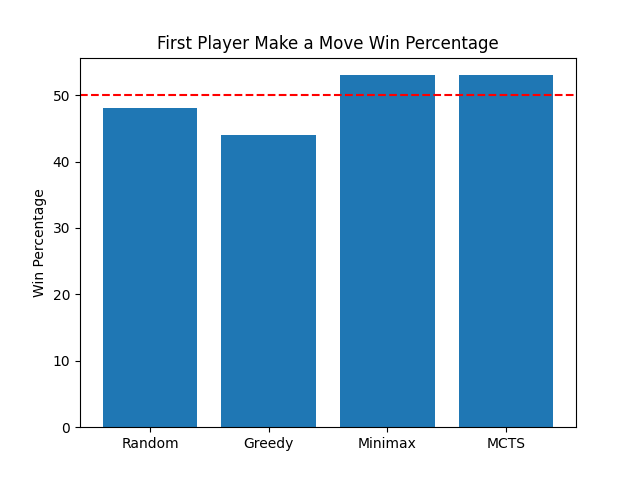
\includegraphics[width=0.8\textwidth]{../img/advantage.png}
  \caption{First player making a move win percentage with Random, Greedy, Minimax, and MCTS}
  \label{firstmoveadvantage}
\end{figure}

The results of the experiment, depicted in Figure \ref{firstmoveadvantage}, indicate that making the first move does not have a significant advantage for basic strategies such as random and greedy. Specifically, the random agents won 48 out of 100 games when making the first move, and the greedy agents won 44 out of 100 games under the same circumstances. On the other hand, more complex strategies such as minimax and MCTS appear to benefit from making the first move, with the minimax agents winning 53 out of 100 games and the MCTS agents also winning 53 out of 100 games. While the results suggest that the first player has a slight advantage when using more advanced strategies and does not have a slight advantage when using the basic strategies, the difference in win rate is not extreme, with the win rate for all strategies hovering around 50\%. Therefore, it can be concluded that making the first move does not have a significant impact on the outcome of the game.cre

\section{Classification}

Durak can be classified as a \textbf{discrete game}. A discrete game is a type of game in which players have a finite number of choices, or actions, that they can take \citep{Gametheory4}. This applies in Durak. Players have a limited number of choices that they can make at each turn. They can choose which card to play, and must decide whether to attack or defend. These choices are limited by the cards that the player has in their hand and the rules of the game. 

Furthermore, it can be considered a \textbf{sequential} game from a game-theoretic perspective. A sequential game is a type of game in which the order in which players make their decisions matters \citep{Gametheory4}. In Durak, the order in which players play their cards is important, as it determines who is able to attack and who must defend. The sequence of actions is determined by the rules of the game described in chapter \ref{GameDescription}, and players must consider the potential actions of their opponents as they make their own decisions. 

In addition, Durak can be classified as a game of \textbf{imperfect information}. In a game of imperfect information, players do not have complete information about the game state or the actions of their opponents \citep{Gametheory4}. They must make decisions based on incomplete information and must try to infer the actions of their opponents based on their observations and past experiences. As described before, Durak is a game of imperfect information because players do not have complete information about the cards in the hands of their opponents. They must make decisions about which cards to play and when to use their trump cards based on incomplete information, and must adapt their strategies as the game progresses and new information becomes available.

Additionally, Durak is often played in a \textbf{deterministic} manner, meaning that the outcome of the game is determined by the initial cards that are dealt and the actions that are taken by the players during the game. However, there is some element of chance in Durak, as the cards are shuffled randomly before the game begins can affect the outcome of the game. Therefore, it is possible to consider Durak to be a \textbf{non-deterministic} game to some degree. In game theory, a non-deterministic game is a type of game in which the outcomes are not determined solely by the actions of the players and the rules of the game, but are also influenced by random events or factors \citep{Gametheory4}. 

In summary, Durak can be classified as a discrete, sequential, imperfect information, and non-deterministic to some extent game from a game-theoretic perspective, which contribute to its complexity and strategic depth.


\section{Branching Factor}

The branching factor of a game refers to the number of possible moves that a player can make at each turn. In ``Podkidnoy Durak'', it can be challenging to determine the branching factor as it varies depending on the specific game state. At each turn, the number of possible moves a player can make is influenced by the cards in their hand and the cards on the table, as well as the defending or attacking rules. To be specific, the attacker can initiate an attack by playing any card from their hand. Therefore, the maximum branching factor is the maximum number of cards that a player can hold in their hand, which is 35 if one player holds all but one of the cards. However, there are also situations in which a player may only have one possible move, such as when they are unable to defend against an attack and must pass and take the card. Therefore, the average branching factor in this game is relatively low, as players often have only a few choices of cards to play in a given situation. This is particularly true for the defender, who may only have a few options for defending against an attack, and for subsequent attacks, where the number of available options may also be limited.

To clarify the branching factor assumption, I have run an experiment to estimate the average branching factor in Durak by simulating 1000 random games played between two greedy agents. The results showed that the average branching factor, as computed using the \textbf{geometric mean}, was \textbf{2.17}, which suggests that the branching factor of the game is low. 

\section{Duration}

The objective of this section is to determine the typical duration of games of Durak in terms of bouts and plies, where ply refers to a single move made by a single player. To address this question, we will compare the average length of games played between two random players and two greedy agents, in order to examine the influence of player strategy on the duration of the game.

To compare the durations of player strategies in Durak, we conducted two experiments. The first experiment involved 1000 games played between two greedy agents, and the second experiment involved 1000 games played between two random agents. The results of the first experiment showed that the average number of bouts per game was 8.3, the average number of plies per bout was 5.3, and the average number of plies per game was 44.0. The results of the second experiment showed that the average number of bouts per game was 24.0, the average number of plies per bout was 2.9, and the average number of plies per game was 68.0. These findings suggest that the behavior of the random agents led to longer games, as evidenced by the higher number of bouts and lower number of plies per bout in the second experiment.

\section{Weakness Concept}
\label{weaknessConcept}
This section introduces the concept of \textbf{weakness} and \textbf{well-covered weakness} in Durak, which are the concepts that arise from the analysis of the game and may be relevant to various strategies or agents.

The concepts in question are introduced in Edouard Bonnet's paper ``The Complexity of Playing Durak''. It examines the difficulty of identifying winning strategies in the card game Durak. Bonnet's work demonstrates that, even in a perfect information setting with two players, finding optimal moves is a challenging computational problem. Specifically, Bonnet establishes that determining the presence of a winning strategy in a generalized Durak position is PSPACE-complete \citep{Bonnet2016TheCO}. In my own research, I aim to construct a strong agent capable of playing optimally in both perfect and imperfect information settings. Bonnet's contributions, including the concept of weakness and well-covered weakness, have been invaluable in the development of my rule-based agents.

A weakness for a player, referred to as player \textit{P}, is defined as a rank \textit{r} that meets the following criteria: 
\begin{enumerate}
	\item player \textit{P}'s hand contains at least one card of rank \textit{r}, and
	\item for each suit \textit{s} of rank \textit{r} in player \textit{P}'s hand, there exists a rank $\textit{r}$'$ > \textit{r}$ such that the opponent holds a card of rank \textit{r}$'$ and suit \textit{s} \citep{Bonnet2016TheCO}.
\end{enumerate}

To clarify the concept of weakness, consider the following scenario: Player P holds the cards 10$\textcolor{red}{\heartsuit}$, 10$\textcolor{black}{\spadesuit}$, and K$\textcolor{red}{\diamondsuit}$, while player O holds Q$\textcolor{red}{\heartsuit}$, Q$\textcolor{black}{\spadesuit}$, and J$\textcolor{black}{\clubsuit}$. In this case, player P has a weakness at rank 10, as it satisfies the two conditions outlined in the definition of weakness. Specifically, player P holds at least one card of rank 10 (10$\textcolor{red}{\heartsuit}$ and 10$\textcolor{black}{\spadesuit}$), and for each suit of rank 10 in player P's hand (10$\textcolor{red}{\heartsuit}$ and 10$\textcolor{black}{\spadesuit}$), the opponent holds a card of higher rank (Q$\textcolor{red}{\heartsuit}$ and Q$\textcolor{black}{\spadesuit}$, respectively).

A well-covered weakness for player \textit{P}, on the other hand, refers to a weakness card with rank \textit{r} such that for every card in player \textit{P}'s hand with suit \textit{s} and rank \textit{r}, there is a higher card with suit \textit{s} and rank \textit{r}' in player \textit{O}'s hand, and player \textit{P} does not possess any cards with rank \textit{r}'. Essentially, if player \textit{P} attacks with a well-covered weakness, player \textit{O} can defend effectively, preventing player \textit{P} from playing any other attacking cards during the bout.

In the example provided following the definition of weakness, the cards 10$\textcolor{red}{\heartsuit}$ and 10$\textcolor{black}{\spadesuit}$ are considered well-covered weaknesses because attacking with these cards allows the opponent, player O, to effectively defend with Q$\textcolor{red}{\heartsuit}$ and Q$\textcolor{black}{\spadesuit}$ and prevent player P from attacking again.

\section{Closed World Deduction}

In the closed world environment, it is possible for a player to deduce the opponent's remaining cards once the deck is depleted. This is because once the deck is exhausted, the only cards that can be played are those that are held by the players. If a player is able to keep track of the cards that have been played, they can narrow down the possible cards that their opponent still holds and make educated guesses about their strategy based on this information. To give an example, imagine that the deck has been exhausted, and there are only four cards left in the game: A$\textcolor{red}{\heartsuit}$, 6$\textcolor{black}{\spadesuit}$, 7$\textcolor{red}{\diamondsuit}$, and 8$\textcolor{black}{\clubsuit}$. Player A is able to deduce that their opponent, player B, still holds A$\textcolor{red}{\heartsuit}$ because they have played the 6, 7, and 8 cards, but have not yet played the A card. Based on this information, player A can infer that player B is likely trying to hold onto the A card in order to use it as a trump card later in the game. By paying a close attention, player A will know which cards have already been played and which ones are still in play. Player A knows that A$\textcolor{red}{\heartsuit}$ has not yet been played because they have not seen it played, and they also know that the A$\textcolor{red}{\heartsuit}$ card has not been discarded because the deck has not yet been exhausted. Therefore, player A can deduce that the A$\textcolor{red}{\heartsuit}$ card is still in play either in the deck or in the opponent's hand. Once the deck is depleted, it becomes obvious that it is being held by player B. The ability to deduce an opponent's remaining cards can significantly impact the course of the game, as it allows players to incorporate this information into their strategic decision-making. However, it is important to note that Durak is a game of chance as well as strategy, and even if a player is able to deduce their opponent's remaining cards, they cannot predict with certainty which cards the opponent will play in a given turn. 